\chapter{מבוא לארכיטקטורות \textenglish{Transformer}}

\section{הקדמה: מהפכה בעיבוד שפה טבעית}

לאורך עשרים השנים האחרונות, עיבוד שפה טבעית (\textenglish{NLP}) התפתח מכלים סטטיסטיים בסיסיים אל תוך מערכות למידה עמוקה המסוגלות לתפוס קשרים סימנטיים מורכבים בטקסט. עם זאת, עד שנת 2017, רוב מודלי הרשתות העמוקות בתחום זה התבססו על \textenglish{Recurrent Neural Networks (RNNs)} וגרסאות משופרות שלהן כמו \textenglish{Long Short-Term Memory (LSTM)} \cite{vaswani2017attention}. למרות יעילותם היחסית, הרשתות הרקורנטיות סבלו מבעיה משמעותית: קשיות בתפיסה של קשרים לטווח ארוך ביותר בטקסט, בגלל בעיית ההתמוטטות והתפוצצות של הגרדיאנטים במהלך ההכשרה.

בשנת 2017, פרסמו ווסוואני וחוקרים נוספים מ-\textenglish{Google} עבודה המשפיעה שכרו \textenglish{"Attention Is All You Need"} --- עבודה שהציגה את ארכיטקטורת \textenglish{Transformer}. דגם חדש זה סילק את הצורך ברקורנציה לחלוטין, וממנו הביא את מנגנון ה־\textenglish{self-attention} לחזית העיצוב. התוצאה הייתה מהפכה: מודלים מתקדמים יותר שיכלו להיות מהופצים ביעילות רבה יותר על פני יחידות עיבוד מרובות (\textenglish{GPU/TPU}), ובעת ובעונה אחת, הם השיגו ביצועים חדישים בשורה של משימות \textenglish{NLP}.

\section{בעיית האילוץ הרקורנטי וקיום הטעם}

רשתות \textenglish{RNN} קלאסיות מעבדות רצפים באופן סדרתי --- כל אלמנט בקלט מעובד רק לאחר עיבוד האלמנט הקודם. עיצוב סדרתי זה יוצר שתי בעיות עיקריות:

\begin{enumerate}
\item \textbf{חוסר הקביל:} בגלל תלות הרקורנציה, לא ניתן לעבד אלמנטים שונים בו־זמנית, מה שהופך הדרכה וחיזוי למבוצעים ממאנים למודלים ארוכים.
\item \textbf{עיוותי קשר לטווח ארוך:} \textenglish{Gradient flow} דרך צעדי זמן רבים גורם לבעיות כמו התמוטטות וריבוי של גרדיאנטים, המקשות על לימוד קשרים בין אלמנטים רחוקים בטקסט.
\end{enumerate}

ארכיטקטורת \textenglish{Transformer} פותרת בעיות אלו בתשומת לב עצמית (\textenglish{self-attention}), המאפשרת לכל אלמנט לקבל קשר ישירות אל כל אלמנט אחר ברצף, ללא רקורנציה. זה פותח את הדלת לעיבוד מקביל מלא וקשרים לטווח ארוך יותר בעקביות.

\section{עדכוני מפתח בארכיטקטורות דגם שפה}

מאז הצגת \textenglish{Transformer}, המחקר בתחום \textenglish{NLP} התרכז על כיוונונים וטוב של עקרונות הבסיס. שלושה מודלים משפיעים יותר זה שלפנינו:

\begin{equation}
\text{Attention}(Q, K, V) = \text{softmax}\left(\frac{QK^{\top}}{\sqrt{d_k}}\right)V
\end{equation}

\textenglish{BERT} \cite{devlin2019bert} הטמיע \textenglish{Transformers} דו-כיווניים עם הדרכה קדם-מטלה על קורפוסים ענקיים, והשיג ביצועים טובים ביותר בעשרות משימות \textenglish{downstream}. בעקבות זה, דגמים גדולים יותר כמו \textenglish{GPT-2} \cite{brown2020language} הדגימו שעם הרחבה של נתוני הדרכה וגודל דגם, ניתן להשיג אבדות פחותות ביותר בחיזוי הטוקן הבא. \textenglish{GPT-3} \cite{radford2019language} הוריד הדגמה זו לקיצוניותה, והראה שמודלים בגודל מרה־גדול יכולים לעונות על משימות חדישות עם רק כמה דוגמאות או בלעדיהן (\textenglish{few-shot} ו-\textenglish{zero-shot learning}).

\begin{figure}[H]
\centering
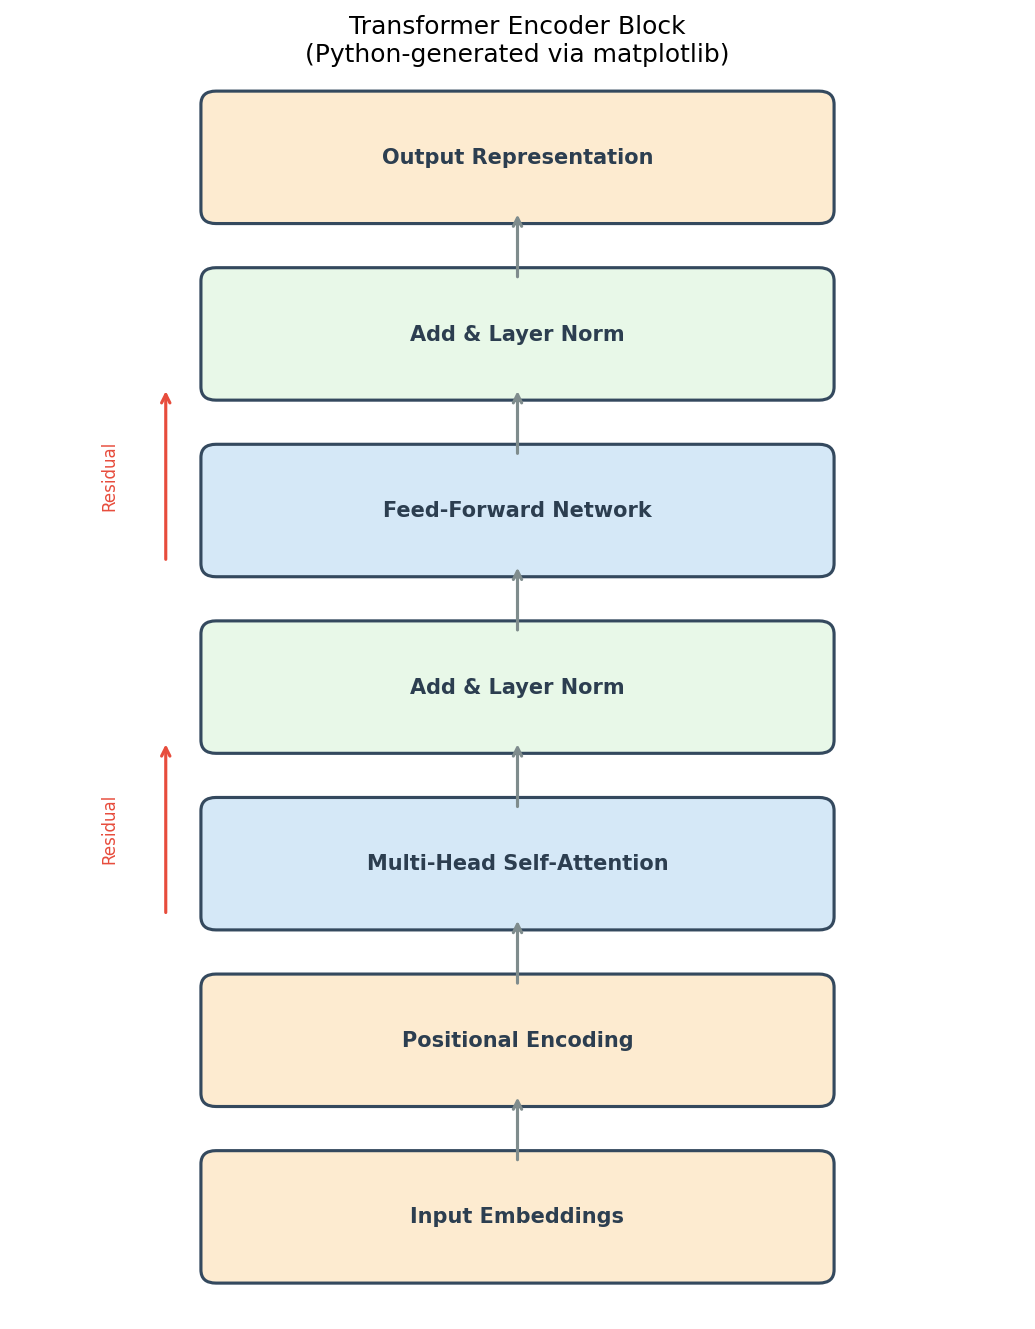
\includegraphics[width=0.72\textwidth]{assets/transformer_architecture.png}
\caption{\textenglish{Transformer Encoder Block Diagram (Python-generated)}}
\label{fig:transformer_architecture}
\end{figure}

\section{יעדים ותרומות של הספר הזה}

כתאב זה מוקדש לחקר מעמיק של ארכיטקטורות \textenglish{Transformer} והיישומים שלהן בעיבוד שפה טבעית. אנחנו נחקור:

\begin{itemize}
\item את המיכניקה המפורטת של מנגנון ה-\textenglish{self-attention}
\item את תפקיד ה\textenglish{-positional encoding} בהעברת מידע מיקום
\item את ההבדלים בין \textenglish{encoder} לבין \textenglish{decoder} ארכיטקטורות
\item דוגמאות מעשיות לדרך יישום מודלים אלו
\end{itemize}

בנוסף, נשקול השפעות הנדסיות כמו יעילות זיכרון, שיפור הדרכה, ופתרונות עבור רצפים ארוכים מאוד. הקוראים יצאו מכתאב זה בעלי הבנה עמוקה לא רק איך \textenglish{Transformers} עובדים, אלא למה הם משדרגים שיטות קודמות וכיצד הם מהווים הבסיס לדור חדש של מערכות בינה מלאכותית.
